\section{Mapping URIs to zipper-based paths and back}

\subsection{Path and context}

\subsection{Homomorphisms and obfuscation}

\section{Applying zippers to our project}

\begin{figure}[tbp]
\begin{center}
{ 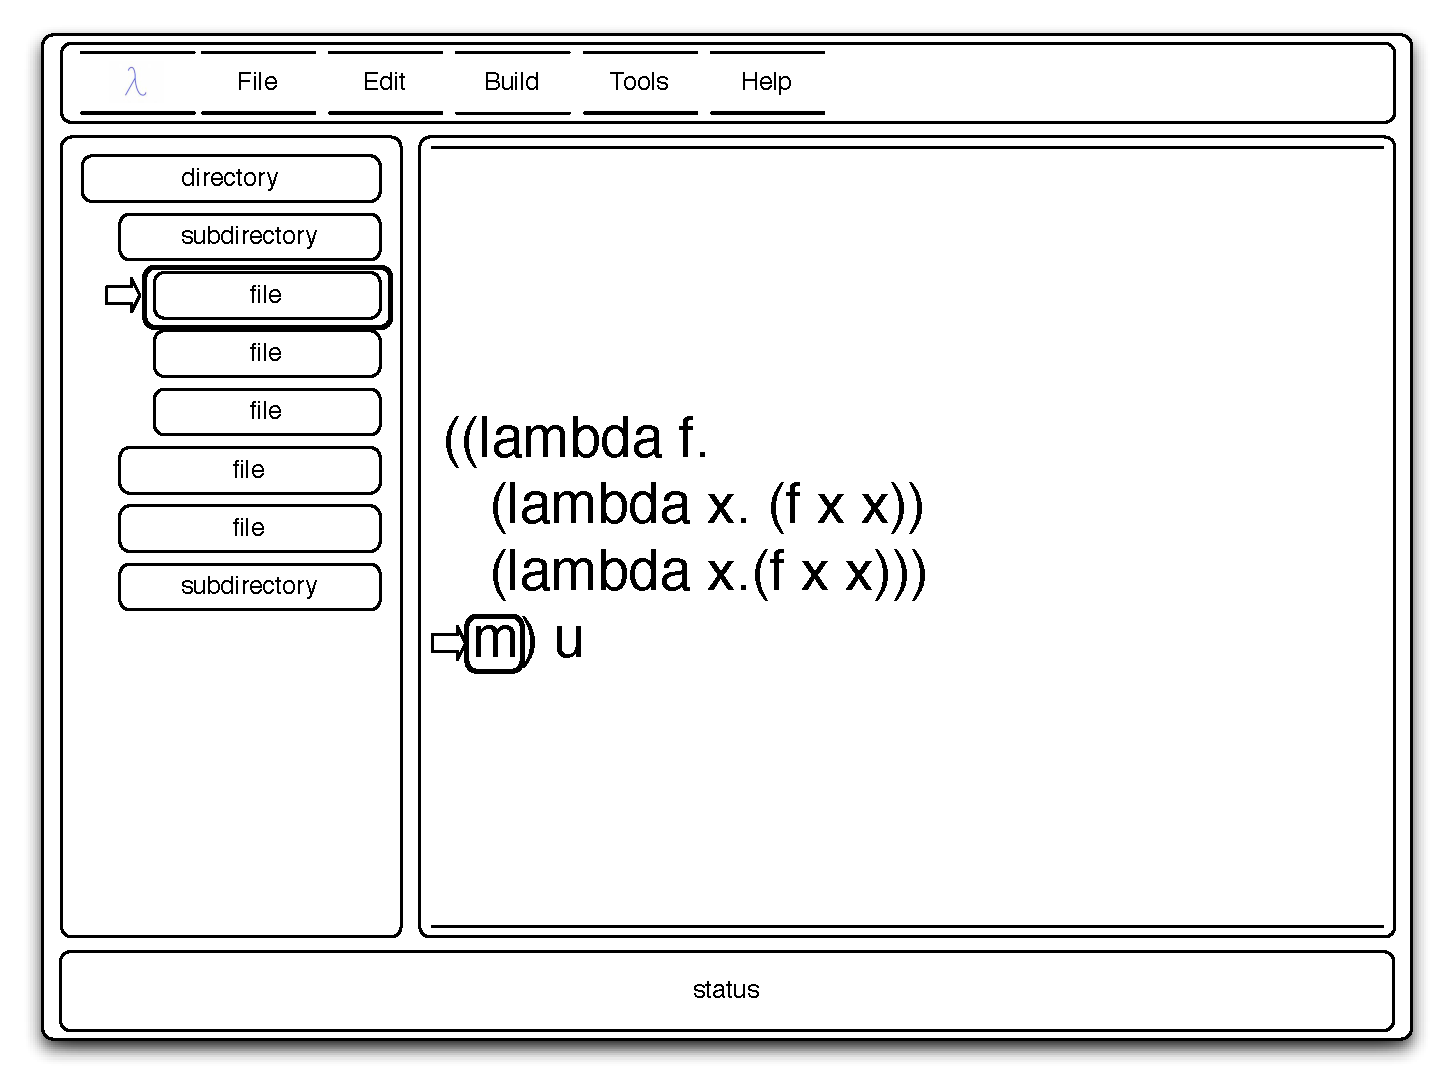
\includegraphics[scale=.65]{/Users/lgm/work/src/projex/biosimilarity/trace/src/main/book/content/figures/ProjectZipper.pdf} }
\caption{ Zippers and editors }
\end{center}
\end{figure}
\subsection{Navigating and editing terms}

Consider the following term.

\begin{lstlisting}[language=Scala,mathescape=true]
  // Corresponds to the Church numeral: 
  // $\lambda \; f . \; \lambda \; x . $
  //     $(f \; \lambda \; f . \; f \; \lambda \; f \; . \; \lambda \; x . \; x )$
  //     $((f \; \lambda \; f \; . \; \lambda \; x . \; x) x)$ 
  Abstraction(
    List( StringLiteral( "f" ) ),
    Abstraction(
      List( StringLiteral( "x" ) ),
      Application( 
        Application(
          Mention( StringLiteral( "f" ) ),
          Abstraction( 
            List( StringLiteral( "f" ) ),
            Application( 
              Mention( StringLiteral( "f" ) ),
              Abstraction(
                List( StringLiteral( "f" ) ),
                Abstraction(
                  List( StringLiteral( "x" ) ),
                  Mention( StringLiteral( "x" ) )
                )
              )
            )
          )
        ),
        Application(
          Application( 
            Mention( StringLiteral( "f" ) ),
            Abstraction(
              List( StringLiteral( "f" ) ),
              Abstraction(
                List( StringLiteral( "x" ) ),
                Mention( StringLiteral( "x" ) )
              )
            )
          ),
          Mention( StringLiteral( "x" ) )  
        )
      )
    )
  )
\end{lstlisting}

\subsection{Navigating and editing projects}
